\documentclass[pdftex,10pt,a4paper,oneside]{article}

\usepackage{amsmath}
\numberwithin{equation}{section}
\usepackage{algorithm}
\usepackage{algorithmic}
\usepackage{fancyhdr}
\usepackage{graphicx}
\usepackage{setspace}
\usepackage[]{fncychap}
\usepackage[hyphens]{url}
\usepackage{xcolor}
\usepackage{tabularx}
\usepackage{appendix}
\usepackage[hidelinks]{hyperref}
\usepackage{pdfpages}
\usepackage[round]{natbib}
\usepackage[a4paper,margin=1in]{geometry}
\usepackage{longtable}
\usepackage{caption}

% Fancy header/footer
\fancyhf{}
\pagestyle{fancy}
\renewcommand{\headrulewidth}{0.2pt}
\fancyfoot[C]{\thepage}

% Begin document
\begin{document}

% Preamble
 % Remove headers/footers for the title page
\thispagestyle{empty}

% Double spacing for the title page
\begin{spacing}{2}
    \begin{center}

        % University Crest
        
\includegraphics[scale=0.45]{preamble/warwick-crest.pdf}
        \vspace{10mm}

        % Dissertation Title
        \textbf{\LARGE AI Phishing Detection with Explainable AI}
        \vspace{20mm}

        % Student ID
        {\large \textbf{Student ID: 2242090}}
        \vspace{20mm}

        % Supervisor and Department
        {\large Supervisor: Sarah Aktaa}\\
        \textbf{\large Department of Warwick Manufacturing Group (WMG)}\\
        {\large University of Warwick}\\
        {\large Academic Year: 2024-2025}

    \end{center}
\end{spacing}

% Start Roman numbering for front matter
\pagenumbering{arabic}

\newpage
% ai-phishing-detection-dissertation/report/preamble/abstract.tex

\section*{Abstract}
\addcontentsline{toc}{section}{Abstract}

Phishing attacks are known to be a big challenge in cybersecurity. Whilst Artificial Intelligence (AI) can help in detecting and preventing such attacks, most models are "black-boxed", and this limits user trust. This study therefore researches the practical development of an AI-powered phishing detection by implementing and evaluating two distinct models: a Random Forest classifier with TF-IDF features and a fine-tuned DistilBERT transformer. Explainable AI (XAI) techniques, such as SHAP for Random Forest and LIME for DistilBERT, were integrated to enhance model transparency. Both models achieved high accuracies of over 98\% on an internal test set comprised of Enron and CEAS 08 corpora. Evaluations on independent, extenal datasets (SpamAssassin, Nigerian Fraud, Nazario) revealed generalisation challenges. Although there was a high precision for phishing instances, there was equally as low recall. The XAI methods integrated provide both global and local explanations, showing how features and words contributed to the model's final outcome.\newline

\large
\noindent This project aligns with the following CyBok Skills: \textbf{Malware \& Attack Technologies}, \textbf{Human Factors}, \textbf{Adversarial Behaviours}.
\newpage
\section*{Acknowledgements}
\addcontentsline{toc}{section}{Acknowledgements}


\newpage
% ai-phishing-detection-dissertation/report/preamble/abbreviations.tex

\section*{Abbreviations}
\addcontentsline{toc}{section}{Abbreviations}

\large
Artificial Intelligence \hfill AI\\
Anti-Phishing Working Group \hfill APWG\\
Challenge Lab Evaluation Corpus \hfill CEAS\\
Deep Learning \hfill HL\\
Explainable Boosting Machines \hfill EBM\\
General Data Protection Regulation \hfill GDPR\\
Global Digital Population \hfill GDP\\
Gated Recurrent Unit Long Short-Term Memory \hfill GRU-LSTM\\
K-Nearest Neighbours \hfill KNN\\
Large Language Model \hfill LLM\\
Local Interpretable Model-agnostic Explanations \hfill LIME\\
Machine Learning \hfill ML\\
Natural Language Processing \hfill NLP \\
SHapley Additive exPlanations \hfill SHAP\\
Simple Vector Machine \hfill SVM\\
Uniform Resource Locator \hfill URL\\
Voice over Internet Protocol \hfill VoIP\\
eXplainable Artificial Intelligence \hfill XAI\\
eXplainable Artificial Intelligence with\newline Aquila Optimization Algorithm in Web Phishing Classification \hfill XAIAOA-WPC\\
eXplainable Artificial Intelligence Ensemble-based Filter Feature Selection \hfill XAI-EFFS\\
University of New Brunswick \hfill UNB\\


\newpage
% ai-phishing-detection-dissertation/report/preamble/contents.tex

\setcounter{tocdepth}{2}
\tableofcontents


\newpage
% ai-phishing-detection-dissertation/report/preamble/lists.tex

\listoffigures
\addcontentsline{toc}{section}{List of Figures}
\numberwithin{figure}{section}

\listoftables
\addcontentsline{toc}{section}{List of Tables}
\numberwithin{table}{section}

\listofalgorithms
\addcontentsline{toc}{section}{List of Algorithms}
\numberwithin{algorithm}{section}


\newpage
\pagenumbering{arabic}

\lfoot{\centering \thepage}

\newpage

% Sections
\section{Introduction}\label{sec:1-introduction}
\subsection*{Background}

It is deemed that phishing attacks are one of the most common forms of cyber crimes today, with its targets ranging from individuals to large-scale organisations, with the aim of obtaining sensitive information including personal identification, credentials, and financial data. Acording to the DataBreach Report by \cite{verizon2023}, it was investigated that social engineering was responsible for over 50\% of all breaches -- a significant point to consider for cybersecurity. The attacks mainly use complex social engineering techniques such as deceptive content, malicious URLs posing as legitimate, and impersonation, all in an attempt to bypass traditional security systems \citep{marett2009effectiveness}. \newline

\noindent Therefore, Artificial intelligence (AI) and machine learning (ML) can serve as effective tools in detecting phishing attempts. Models can be trained on huge datasets on features like suspicious email headers, text anomalies, and malicious links, which humans have a high probability of missing (\cite{chandrasekaran2006phoney}; \cite{jain2022survey}). However, it is important to note that most traditional AI-phishing detection systems function as a "black-box" model, and they don't offer much transparency into their decision-making processes. Since there is little to no interpretability, it not only reduces trust on the user's side, but the risk that these systems carry inhibit it from being implemented in high-stakes environments such as financial institutions and governmental agencies \citep{ribeiro2016model}. \newline

\noindent Explainable AI (XAI) solve this challenge by attempting to make AI systems more understandable and transparent. Techniques like SHAP (SHapley Additive Explanations) and LIME (Local Interpretable Model-agnostic Explanations) can give insights into the prediction process models undergo (\cite{lundberg2017unified}; \cite{ribeiro2016model}). Especially for phishing detection, XAI can very much empower a user's confidence in understanding why an email is flagged, due to either language cues, suspicious links, or email metadata. \newline

\noindent However despite advances in AI and XAI, there still remain gaps into integrating explainability into phishing detection models. Many existing approaches have a prioritisation on accuracy, without much thought for comprehensability \citep{hernandes2021phishing}. This means its difficult to strike a balance between performance and transparency. This project therefore addresses to seek this gap, by developing an XAI-enhanced phishing detection system that achieves a high accuracy whilst providing actionable explanations behind its predictions.

% ai-phishing-detection-dissertation/report/sections/1-introduction/objectives.tex

\subsection{Objectives}

\begin{enumerate}
  \item \uline{\textbf{OBJECTIVE 1}}: "\textit{Conduct a comprehensive review of existing AI phishing detection models}.\label{objective-1}"
  \begin{itemize}
    \item Review existing AI phishing detection systems.
    \item Identify research gaps to address in relation to interpretability in phishing detection.
    \item Explore XAI techniques, like SHAP and LIME, and their applicability for phishing detection
    \end{itemize}
  \item \uline{\textbf{OBJECTIVE 2}}: "\textit{Identify and implement suitable XAI techniques (e.g., SHAP, LIME)}.\label{objective-2}"
  \begin{itemize}
    \item Develop upon a traditional model already being used for phishing detection, e.g. Random Forest or Transformer-based models.
    \item Integrate XAI techniques into these models that can explain the model predictions.
    \item Achieve a competitive accuracy that is either on par or better than existing AI-based phishing detection models.
  \end{itemize}
\item \uline{\textbf{OBJECTIVE 3}}: "\textit{Evaluate the system's performance in terms of accuracy and interpretability}.\label{objective-3}"
  \begin{itemize}
    \item Assess the system on performance metrics such as precision, accuracy, and recall.
    \item Analyse how useful explanations are using standard interpretability metrics.
  \end{itemize}
\item \uline{\textbf{OBJECTIVE 4}}: "\textit{Compare the usability of the XAI phishing detection model with traditional black-boxed models}.\label{objective-4}"
  \begin{itemize}
    \item Conduct small-scale user studies or surveys to determine how effective XAI influences usability and trust -- compared to black-boxed phishing detection models.
    \item Discuss whether or not its worth compromising on accuracy to achieve trust and usability.
  \end{itemize}
\end{enumerate}

\subsection*{Research questions}

\begin{enumerate}
    \item \textbf{Primary research question:}
        \begin{itemize}
            \item \textit{How can Explainable AI (XAI) improve the usability and trustworthiness of AI-based phishing detection systems without compromising on accuracy?}
        \end{itemize}
    \item \textbf{Sub-questions:}
        \begin{itemize}
            \item What are the current limitations of AI phishing detection models in terms of their usability and interpretability?
            \item How do the interpretability features affect a user's trust building and decision-making processes?
            \item How can XAI techniques, i.e. SHAP and LIME, be integrated efficiently on top of existing AI phishing detection models?
            \item What trade-offs, if any, arise between the performance and interpretability of the AI phishing detection model?
        \end{itemize}
\end{enumerate}

\subsection*{Paper structure}

The paper is structured as follows: \hyperref[sec:2-literature-review]{Section 2} is the result of a comprehensive literature review into the space of AI-based phishing detection, which neatly progresses onto the relevance of XAI in this field. \hyperref[sec:3-research-methodology]{Section 3} discusses the research methodology, and the practical implementation of the XAI-enhanced phishing detection model.


\newpage

\section{Literature review}\label{sec:2-literature-review}
% ai-phishing-detection-dissertation/report/sections/3-research-methodology/model-development/introduction.tex


\subsection*{AI-based phishing detection models}

% ai-phishing-detection-dissertation/report/sections/2-literature-review/challenges-in-ai-based-phishing-detection.tex

\subsection*{Challenges in AI-based phishing detection}

Some simpler models, such as decision trees and random forest, are seen to suffer from a case of overfitting due to the imbalance of datasets and high dimensional data, demonstrated in a study by \cite{harikrishnan2018machine}. A large majority of the reasons as to the performance drop-off is due to dataset limitations like lack of specific features or dataset size, as observed by \cite{ahmad2024across}. They mainly noted how datasets struggled to perform well due to a lack of quality and diverse data. Training times were a significant challenge, not just from dataset size, but the inherent nature of deep learning models (consisting of many layers), that might limit their applicability in real-time situations, as discovered by \cite{kapoor2024comparative}, which is also agreed upon by \cite{atlam2022business}. In \cite{kapoor2024comparative}'s research, they also comment on the constant evolution of sophisticated tactics introduced by attackers, such a deep fakes, new social enginnering tactics, and context-aware attacks -- all with the goal of exploiting human technology. They mention that it is important to factor in an "arms race" between AI models being trained on new data and attackers coming up with new intrusion methods. Traditional models, apart from overfitting, suffer from their sensitivity to parameter turning such as SVM \citep{andriu2023adaptive}. Furthermore, it is a challenge to scale these models given the ever-growing needs of an organisation, as the system must be able to both maintain its performance and optimal detection to deal with increasing workloads, with a lack of real-time implementations and studies, observed by \cite{atlam2022business}. GDPR comes into play here as these systems use user information from email content and metadata, so they need to be ensure compliance and have the appropriate privacy mechanisms implemented. Models are also likely to fall victim of flagging false positives and negatives, and this is a vital aspect in keeping them from being deployed in a real-time setting, emphasised by \cite{vishwanath2011people}. False positives can logically cause disruption and inconvenicnce for businesses and users respectively, where as false negatives are phishing emails that may bypass filters introducing a vulnerability. It is vital for models to prioritise a balance between these two categories of errors for a practical phishing detection system. Another key area is interpretability challenges mentioned by \cite{atlam2022business}, as they state how most AI models are "black-boxed" from users. Only input and output data can be seen, but the process in between are often obscured. The authors drive forward the point of introducing XAI to allow these models to be interpretable, lading to more dependence and instill a sense of confidence in their decisions. There are other studies, such as by \cite{al2024novel}, that note the challenges associated with interpreting feature importance with non-linear models. But the novelty of XAI in general poses several questions which are addressed in the study by \cite{yakandawala2023review}, where several XAI challenges are listed. The most notable being able to strike the perfect balance between explainability and performance. A model that is non-explainable can recieve "public backlash" due to AI errors and biases, lessening trust in their decision making processes. This especially affects deep learning models which face a lot more interpretability issues than other models due to their complexity. A study to complement this, by \cite{reddy2023explainable}, that suggest several more issues concerning interpretability, such a lack of a universal standard or rigid framework in which to develop and evaluate these XAI techniques. The authors claim that is it important to take human factors into account, and it would prove to be effective to understand how users would interact with such explanations. Additionally, there are also ethical issues, as presented by \cite{hanif2021survey}, that cover areas such as accountability, responsibility, transparency, fidelty, bias, casuality, safety, and fairness -- all concerning XAI explanations.

\subsection*{Explainable AI (XAI) and its relevance to phishing detection}
\subsection*{Existing research on XAI for phishing detection}

\subsection*{Research gaps and justification for this study}

\newpage

\section{Research methodology}\label{sec:3-research-methodology}
\newpage

% References
\bibliographystyle{agsm}
\bibliography{bibliography}
\newpage

% Appendices
\section*{Appendices}
\addcontentsline{toc}{section}{Appendices}

\subsection*{Appendix 1: Ethical approval form}
\addcontentsline{toc}{subsection}{Appendix 1: Ethical approval form}
\label{sec:Appendix 1}

\includepdf[pages=-,scale=0.75]{images/ethical-approval-form.pdf}

\newpage

\subsection*{Appendix 2: Ethical courses certificates}
\addcontentsline{toc}{subsection}{Appendix 2: Ethical courses certificates}
\label{sec:Appendix 2}

\begin{figure}[htbp]
    \centering
    
\includegraphics[width=0.5\textwidth]{images/ethics-in-research-badge.png}
    \caption{Ethics in research badge}
\end{figure}

\begin{figure}[htbp]
    \centering
    
\includegraphics[width=0.5\textwidth]{images/ethical-approval-process-badge.png}
    \caption{Ethical approval badge}
\end{figure}

\begin{figure}[htbp]
    \centering
    \includegraphics[width=1\textwidth]{images/epigeum-certificate.png}
    \caption{Epigeum certificate}
\end{figure}

\begin{figure}[htbp]
    \centering
    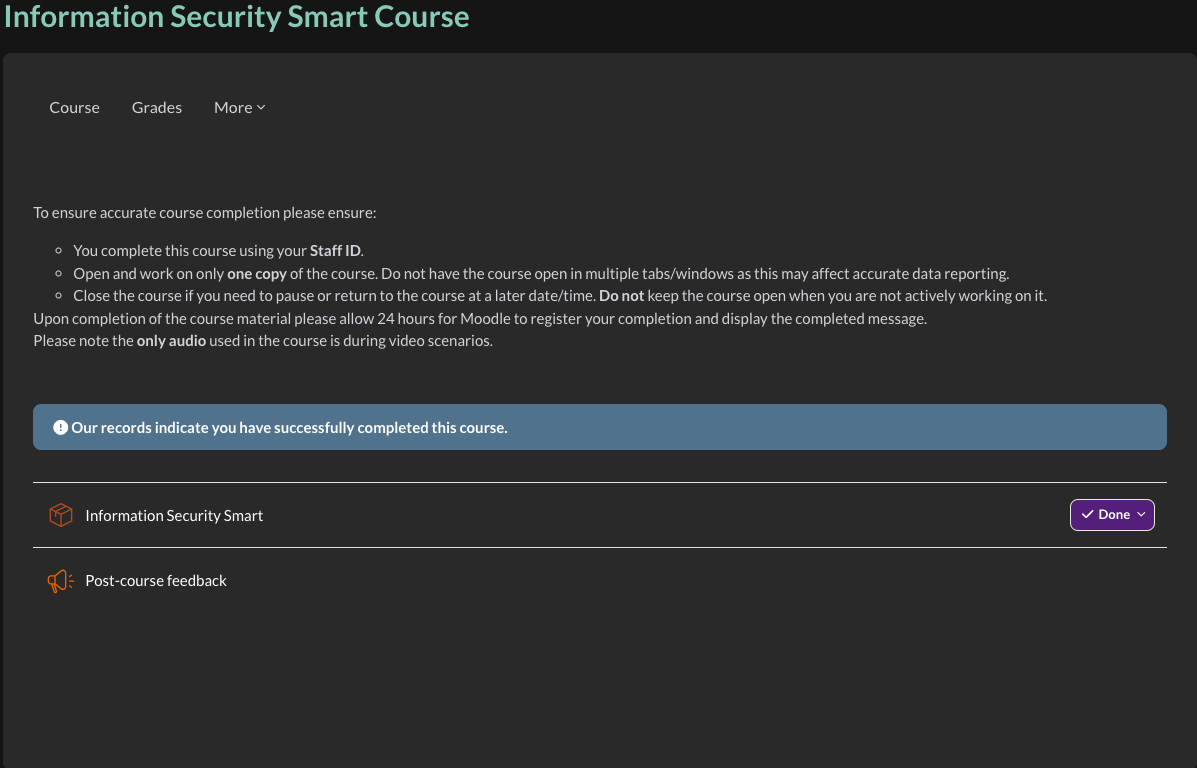
\includegraphics[width=1\textwidth]{images/information-security-smart-certificate.png}
    \caption{Information SMART certificate}
\end{figure}

\newpage

\subsection*{Appendix 3: Project plan}
\addcontentsline{toc}{subsection}{Appendix 3: Project plan}
\label{sec:Appendix 3}

\begin{longtable}{|p{5cm}|p{6cm}|p{4cm}|}
    \hline
    \textbf{Phase} & \textbf{Tasks} & \textbf{Duration} \\
    \hline
    \endfirsthead
    \hline
    \textbf{Phase} & \textbf{Tasks} & \textbf{Duration} \\
    \hline
    \endhead
    
    \hline
    \endfoot
    
    \hline
    \endlastfoot
    
    Research and Planning & 
    \begin{itemize}
        \item Conduct literature review.
        \item Refine research questions and objectives.
        \item Identify datasets (e.g., PhishTank, Kaggle).
    \end{itemize} & 
    End Jan – Early Feb (1–2 weeks) \\
    \hline
    
    Dataset Preparation & 
    \begin{itemize}
        \item Clean and preprocess data.
        \item Perform feature extraction (e.g., URLs, metadata).
        \item Split data into training, validation, and test sets.
    \end{itemize} & 
    Early Feb (1–2 weeks) \\
    \hline
    
    Model Development & 
    \begin{itemize}
        \item Develop baseline model (e.g., Random Forest, Logistic Regression).
        \item Experiment with advanced models (e.g., BERT).
        \item Train and validate models.
    \end{itemize} & 
    Mid-Feb – Early Mar (3 weeks) \\
    \hline
    
    Integration of XAI & 
    \begin{itemize}
        \item Implement SHAP and LIME for interpretability.
        \item Visualize explanations (e.g., feature importance, email components).
        \item Ensure explanation clarity and usability.
    \end{itemize} & 
    Early Mar – Mid-Mar (2 weeks) \\
    \hline
    
    Evaluation and Comparison & 
    \begin{itemize}
        \item Evaluate model performance (accuracy, F1-score).
        \item Assess interpretability using metrics (faithfulness, stability).
        \item Compare XAI-enhanced system to black-box models.
    \end{itemize} & 
    Mid-Mar – End Mar (2 weeks) \\
    \hline
    
    Report Writing & 
    \begin{itemize}
        \item Write methodology, results, and discussion sections.
        \item Proofread and finalize dissertation.
        \item Integrate appendices (e.g., Gantt chart, ethical approval).
    \end{itemize} & 
    April – Mid-May (5–6 weeks) \\
    \hline
    
    \end{longtable}
    


\end{document}
